%%%%%%%%%%%%%%%%%%%%%%%%%%%%%%%%%%%%%%%%%
% Beamer Presentation
% LaTeX Template
% Version 1.0 (10/11/12)
%
% This template has been downloaded from:
% http://www.LaTeXTemplates.com
%
% License:
% CC BY-NC-SA 3.0 (http://creativecommons.org/licenses/by-nc-sa/3.0/)
%
%%%%%%%%%%%%%%%%%%%%%%%%%%%%%%%%%%%%%%%%%

\documentclass{beamer}
\setbeameroption{hide notes}

% Uncomment these lines (and comment above lines) to print handouts.
% \documentclass[handout]{beamer}
% \setbeameroption{show notes}
% \usepackage{pgfpages}
% \pgfpagesuselayout{4 on 1}[letterpaper,landscape,border shrink=5mm]
% % This makes notes pages totally plain and adds a bit of space between paragraphs on the notes pages.
% \setbeamertemplate{note page}[plain]
% \addtobeamertemplate{note page}{\setlength{\parskip}{12pt}}

%----------------------------------------------------------------------------------------
%	PACKAGES AND THEMES
%----------------------------------------------------------------------------------------

\mode<handout>{

\setbeamercolor{background canvas}{bg=black!5}

}

\mode<presentation> {

% The Beamer class comes with a number of default slide themes
% which change the colors and layouts of slides. Below this is a list
% of all the themes, uncomment each in turn to see what they look like.

%\usetheme{default}
\usetheme{AnnArbor}
%\usetheme{Antibes}
%\usetheme{Bergen}
%\usetheme{Berkeley}
%\usetheme{Berlin}
%\usetheme{Boadilla}
%\usetheme{CambridgeUS}
%\usetheme{Copenhagen}
%\usetheme{Darmstadt}
%\usetheme{Dresden}
%\usetheme{Frankfurt}
%\usetheme{Goettingen}
%\usetheme{Hannover}
%\usetheme{Ilmenau}
%\usetheme{JuanLesPins}
%\usetheme{Luebeck}
%\usetheme{Madrid}
%\usetheme{Malmoe}
%\usetheme{Marburg}
%\usetheme{Montpellier}
%\usetheme{PaloAlto}
%\usetheme{Pittsburgh}
%\usetheme{Rochester}
%\usetheme{Singapore}
%\usetheme{Szeged}
%\usetheme{Warsaw}

% As well as themes, the Beamer class has a number of color themes
% for any slide theme. Uncomment each of these in turn to see how it
% changes the colors of your current slide theme.

%\usecolortheme{albatross}
%\usecolortheme{beaver}
%\usecolortheme{beetle}
\usecolortheme{crane}
%\usecolortheme{dolphin}
%\usecolortheme{dove}
%\usecolortheme{fly}
%\usecolortheme{lily}
%\usecolortheme{orchid}
%\usecolortheme{rose}
%\usecolortheme{seagull}
%\usecolortheme{seahorse}
%\usecolortheme{whale}
%\usecolortheme{wolverine}

%\setbeamertemplate{footline} % To remove the footer line in all slides uncomment this line
%\setbeamertemplate{footline}[page number] % To replace the footer line in all slides with a simple slide count uncomment this line

%\setbeamertemplate{navigation symbols}{} % To remove the navigation symbols from the bottom of all slides uncomment this line
}

\usepackage{graphicx} % Allows including images
\graphicspath{ {./out/img/} }

\usepackage{booktabs} % Allows the use of \toprule, \midrule and \bottomrule in tables

\renewcommand\appendixname{Appendix}

%custom commands

\newcommand{\noi}{\note[item]}

\newcommand{\bei}{\begin{itemize}}
\newcommand{\eei}{\end{itemize}}
\newcommand{\bee}{\begin{enumerate}}
\newcommand{\eee}{\end{enumerate}}

\newcommand{\camp}{\emph{CAMP }}
\newcommand{\campns}{\emph{CAMP}}
\newcommand{\dcamp}{\emph{dCAMP }}
\newcommand{\dcampns}{\emph{dCAMP}}

%----------------------------------------------------------------------------------------
%	TITLE PAGE
%----------------------------------------------------------------------------------------

\title[dCAMP]{Distributed Common API for\\Measuring Performance} % The short title appears at the bottom of every slide, the full title is only on the title page

\author{Alexander P. Sideropoulos} % Your name
\institute[CalPoly] % Your institution as it will appear on the bottom of every slide, may be shorthand to save space
{
California Polytechnic State University, San Luis Obispo \\ % Your institution for the title page
\medskip
\textit{alexander@thequery.net} % Your email address
}
\date{\today} % Date, can be changed to a custom date

\begin{document}

%------------
\begin{frame}
\titlepage % Print the title page as the first slide
\end{frame}

%------------
\begin{frame}
\frametitle{Outline} % Table of contents slide, comment this block out to remove it
\tableofcontents % Throughout your presentation, if you choose to use \section{} and \subsection{} commands, these will automatically be printed on this slide as an overview of your presentation
\end{frame}

%----------------------------------------------------------------------------------------
%	PRESENTATION SLIDES
%----------------------------------------------------------------------------------------

%------------------------------------------------
\section{Introduction}
%------------------------------------------------

%------------------------------------------------
\subsection{Motivation and Scope}

%------------
\begin{frame}
\frametitle{Building Distributed Systems}

Due to the \textbf{plateauing speed} of individual processing units and encouraged by the \textbf{interconnectedness} of
the internet at large, there exists a natural trend of distributing large, complex systems across multiple components
locally and throughout the world.

\note{Notes:}
\noi{cpus not getting faster, but core counts increasing}
\noi{internet has become more pervasive in today's business economy}
\noi{software systems are becoming increasingly distributed}
\noi{EX: large user base --- google, facebook}
\noi{EX: bigger data sets --- ILM, splunk}
\noi{EX: efficient use of resources --- folding@home}
\end{frame}

%------------
\begin{frame}
\frametitle{Building Distributed Systems}

In order to effectively build these systems, software practitioners must be able to test their system for
\textbf{performance defects} as well as bottlenecks, all while the distributed system itself is responding to changes in
availability and work load on its individual nodes.

\note{Notes:}
\noi{systems are not always homogeneous w.r.t. hardware architecture or os}
\noi{development is difficult, even with best tools}
\end{frame}

%------------
\begin{frame}
\frametitle{Distributed Performance Frameworks (DPF)}

Distributed \textbf{Performance Testing} Frameworks:
\bei
\item tools to evaluate performance of system
\item both black box and white box
\item instrumenting, collecting, analyzing, and visualizing distributed performance data
\eei

\medskip

\uncover<2->{
Distributed \textbf{Performance Monitoring} Frameworks:
\bei
\item considered part of the testing framework
\item black box interface
\item monitoring a distributed system or application
\item mechanisms for triggering actions based on performance events
\eei
}

\note{Notes:}
\noi{DPF refers to both}
\end{frame}

%------------
\begin{frame}
\frametitle{Distributed Performance Frameworks (DPF)}
Three types of metric gathering techniques:

\bee
\item hardware counters and sensors use specialized hardware to gather highly accurate metrics and are highly dependent
on the underlying hardware architecture,
\item software sensors use modern operating system interfaces to acquire moderately accurate performance metrics in an
architecture-independent interface, and
\item hybrid approaches use a combination of hardware and software sensors to attain a balance between the two.
\eee

\note{Notes:}
\noi{frameworks listed in this work were chosen based on their categorization in the \cite{zanikolas2005} taxonomy; only
level 2 frameworks are included.}
\noi{Level 2 frameworks are defined as having at least one type of republisher in addition to producers;}
\noi{these frameworks usually distribute functionality across multiple hosts.}
\noi{A limited analysis is conducted by reviewing the available literature, and further analysis (i.e., verifying
scalability, transparency, and validity) is left as future work.}

\end{frame}

%------------------------------------------------
\subsection{Evaluation Criterion}

%------------
\begin{frame}
\frametitle{Criterion for Evaluating Distributed Performance Frameworks}

In order for practitioners and researchers alike to \textbf{effectively choose} a distributed performance framework, it
is necessary to have a set criteria for evaluation. Presented here is an extended criterion of the general requirements
presented by Zanikolas et al. for grid systems \cite{zanikolas2005}.

\bee[<+(1)->]
\item{Data Delivery Models} (original)
\item{Security} (original)
\item{Scalability (only consider good performance)}
\item{Transparency (replaces Low Intrusiveness)}
\item{Extensibility (removed)}
\item{Completeness (new)}
\item{Validity (new)}
\item{Portability (alternate)}
\eee

\note{Notes:}
\noi{there exist several DPF developed by commercial and research institutions}
\noi{\textbf{none found meets all of these criteria}}
\noi{delivery model: periodic vs on-demand (dynamic vs static data), push vs pull (sparse vs stream)}
\noi{security: access control, single or mutual authentication, secure transport of monitoring information}
\noi{transparency: ``typically measured as a function of host (processor, memory, I/O) and network load (bandwidth)
     generated by the collection, processing and distribution of events''}
\noi{portability: run on heterogeneous systems without special considerations; black box}
\end{frame}

%------------------------------------------------
\subsection{Distributed CAMP}

%------------
\begin{frame}
\frametitle{Distributed Common API for Measuring Performance}

\dcamp is a distributed performance framework built on top of Mark Gabel and Michael Haungs' 2007 research on
\emph{CAMP: a common API for measuring performance}\cite{gabel2007}. \camp provides an \textbf{accurate} and
``\textbf{consistent} method for retrieving system performance data from \textbf{multiple platforms}.''

\medskip

\uncover<2->{
\dcamp builds on this functionality and the authors' work validating \campns's accuracy by adding these core feature
sets:

\begin{itemize}
\item stateful performance API
\item distributed performance data aggregation
\item performance filters and triggers
\item simplistic fault tolerance
\end{itemize}
}

\note{Notes:}
\noi{Many authors have failed to address their framework's validity, transparency, and scalability explicitly, thinking
the framework's architecture speaks for itself or blindly assuming it is accurate and introduces negligible load on the
measured system.}
\noi{As shown in the analysis work presented later, \dcamp adds these features while still maintaining minimal impact on the
systems, processes, and networks being monitored.}
\end{frame}

%------------------------------------------------
\section{dCAMP Design}
%------------------------------------------------

%------------------------------------------------
\subsection{Architecture}

%------------
\begin{frame}
\frametitle{System Architecture}

\dcamp is designed as a \textbf{semi-centralized, hierarchical peer-to-peer system} utilizing the UNIX \textbf{Pipes and
Filter} architectural pattern in which leaf nodes of the hierarchy collect data, filter out extraneous data, and send it
up the pipe to a parent node which subsequently filters out more data and sends it up to another parent node.

\note{Notes:}
\noi{This architecture is efficient in that unwanted data is discarded earlier in the data path, reducing transport and
     processing costs.}
\end{frame}

%------------------------------------------------
\subsection{Roles and Services}

%------------
\begin{frame}[t]
\frametitle{\dcamp Roles and Services}

The \dcamp distributed system is comprised of one or more nodes, each executing a \textbf{role}---a named grouping of a
specific, known set of \textbf{services}. Each \dcamp service implements a specific function.

\bei[<+(1)->]
\item \textbf{Node}---rudimentary \dcamp functionality; topology communication, heartbeat monitoring, failure recovery
\item \textbf{Sensor}---local metric gathering; essentially the \dcamp layer on top of OS/hardware APIs (via CAMP)
\item \textbf{Filter}---metric filtering; throttling and thresholding
\item \textbf{Aggregation}--—metric aggregation; metric collection and calculation of multiple Sensor and/or Aggregation services
\item \textbf{Management}--—end-user control of \dcamp 
\item \textbf{Configuration}--—configuration replication; topology and configuration distribution
\eei

\note{Notes:}
\noi{Roles have little to no actual run-time logic but simply act as containers for the services}
\noi{services manage ZeroMQ sockets, communicating with other services/nodes, and do the real work of \dcamp}
\end{frame}

%------------
\begin{frame}[t]
\frametitle{\dcamp Roles and Services}

The \dcamp distributed system is comprised of one or more nodes, each executing a \textbf{role}---a named grouping of a
specific, known set of \textbf{services}. Each \dcamp service implements a specific function.

\medskip

A service's scope can vary depending on the node's level in the \dcamp topology. 
\bei
\item \textit{Root}: master copy of the configuration, publishing new values as needed
\item \textit{Collector}: stores (and forwards) every update from the \textit{Root}
\item \textit{Metric}: only stores updates relevant to the node
\eei

\note{Notes:}
\end{frame}

%------------
\begin{frame}[t]
\frametitle{\dcamp Roles and Services}

The \dcamp distributed system is comprised of one or more nodes, each executing a \textbf{role}---a named grouping of a
specific, known set of \textbf{services}. Each \dcamp service implements a specific function.

\begin{table}
\begin{tabular}{l l}

\hline
\textbf{Role} & \textbf{Service(s)} \\
\hline

Root & Management, Aggregation, Filter, Configuration (Full) \\

Collector & Aggregation, Filter, Configuration (Full) \\

Metric & Sensor, Filter, Configuration (Partial) \\

Base & Node \\

\end{tabular}
\label{tab:role_to_services}
\end{table}

\note{Notes:}
\noi{\textit{Metric} role runs on the nodes from which performance metrics should be collected.}
\noi{\textit{Collector} role acts as an aggregation point in the system, from multiple \textit{Metric} (and
     \textit{Collector}) nodes; provides additional aggregated performance metrics.}
\noi{only one \textit{Root} role; acts as master copy of the configuration and sole user-interface point.}
\noi{\textit{Root} role is not strictly attached to any given node in the system; any first-level \textit{Collector}}
\noi{may choose to split roles across multiple nodes or collapse them onto a single node.}
\end{frame}

%------------
\begin{frame}
\begin{columns}

\begin{column}{6cm}
\begin{figure}[H]
    \centering
    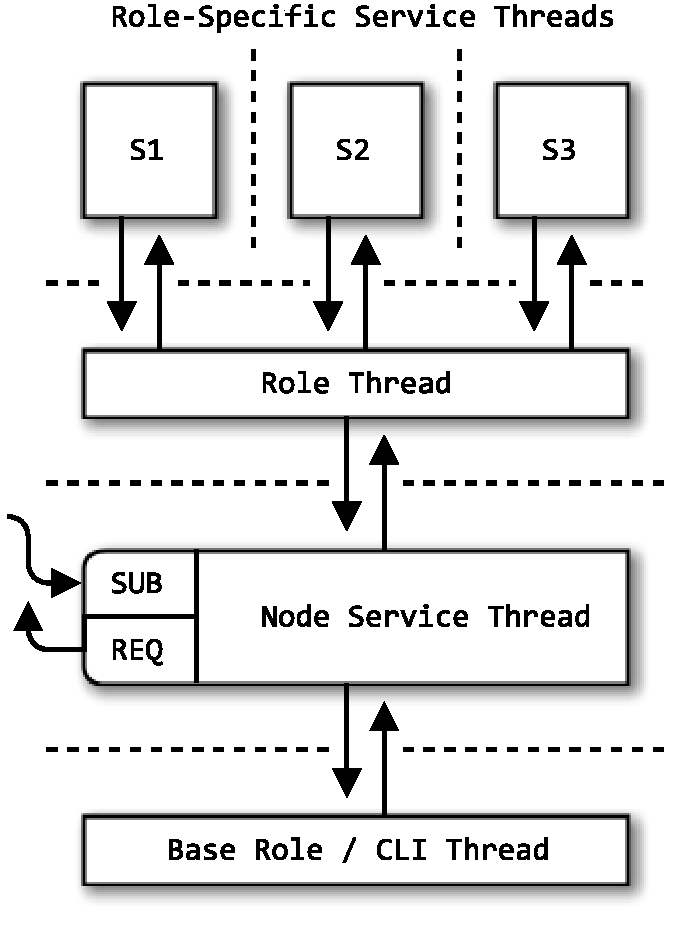
\includegraphics[scale=0.5]{node-role-service.pdf}
    \label{fig:node_role_service_image}
\end{figure}
\end{column}

\begin{column}{5cm}
The \textit{Base} role must be running on each node for it to be part of the \dcamp distributed system. All other roles
are launched from within the \textit{Base} role.
\end{column}

\note{Notes:}
\noi{In this document, a ``\textit{Base} node'' is defined as a \dcamp node which has not yet been configured, i.e. it
     has not joined a running \dcamp system.}
\noi{Node, Role, Services Threading Model Diagram: Thread boundaries are represented by dashed lines. Except for the
     Node service's \texttt{SUB} and \texttt{REQ} sockets, all arrows represent \texttt{PAIR} socket communication.}
\noi{\textit{Base} node can transform into one of the three active \dcamp roles; this transformation is actually the
     \textit{Base} role (via the Node service) launching and managing another role internally.}
\noi{When a \textit{Base} node, only bottom two threads (\textit{Base} and Node) are active.}
\noi{after assignment from the ``discover'' Topology Protocol or CLI, Node service launches an appropriate role thread
     which, in turn, launches one or more role-specific service threads.}
\noi{also various service-to-service communications via \texttt{inproc} sockets (e.g. internal Data Flow Protocol) and
     shared memory (e.g. the Configuration service).}

\end{columns}
\end{frame}

%------------------------------------------------
\subsection{Operation}

%------------
\begin{frame}
\frametitle{Sequence of \dcamp Operation}

\bee[<+->]
\item User promotes a \textit{Root} node via the \dcamp CLI, specifying a configuration file and a \textit{Base} node's
      address.
\item \textit{Root} node connects to each \textit{Base} node and begins the ``discover'' Topology Protocol.
\item \textit{Base} nodes join the \dcamp system at any time, being assigned as \textit{Collector} or \textit{Metric}
      nodes in the topology.
\item \dcamp runs in a steady state, nodes entering or exiting the system at any time.
\item User stops \dcamp by using the \dcamp CLI command.
\item \textit{Root} node begins the ``stop'' Topology Protocol.
\item \textit{Collector} and \textit{Metric} nodes exit the topology and revert to \textit{Base} nodes.
\item \textit{Root} node exits, reverting to \textit{Base} node.
\eee

\note{Notes:}
\noi{\textit{Base} nodes (other \textit{Root}) can be started at any time by using the \dcamp CLI}
\noi{expected \textit{Base} nodes are managed by a watchdog utility}
\end{frame}

%------------
\begin{frame}
\frametitle{Steady-State Operation}
\bee[<+->]
\item Performance counters are sampled, filtered, reported, and logged by the Metric nodes at regular intervals
      according to the \dcamp Configuration.
\item Performance counters received from child nodes are aggregated, filtered, reported, and logged by
      \textit{Collector} nodes at regular intervals according to the \dcamp Configuration.
\item Performance counters received from child nodes are aggregated and logged by \textit{Root} node for later
      processing (e.g. graphing metrics during a test scenario or correlating statistics with a distributed event
      log).
\eee

\note{Notes:}
\end{frame}

%------------------------------------------------
\section{dCAMP Details}
%------------------------------------------------

%------------------------------------------------
\subsection{ZeroMQ Protocols}

%------------
\begin{frame}[t]
\frametitle{Topology Protocol}
The \dcamp distributed topology is dynamically established as the \textit{Root} node sends out its discovery message and
receives join messages from \textit{Base} nodes. When a \textit{Base} node responds to the \textit{Root}, the
\textit{Base} node is given its assignment.

\centering
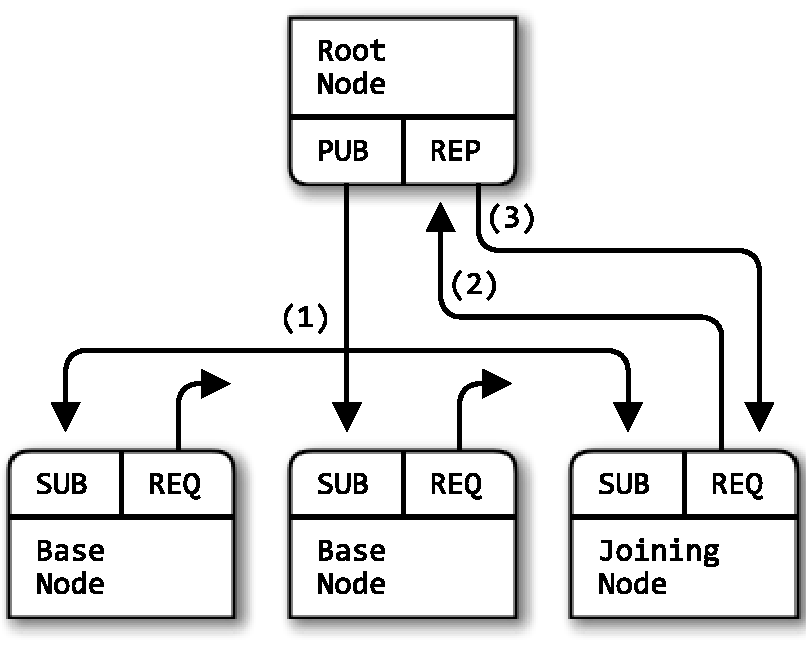
\includegraphics[scale=0.5]{topo.pdf}

\note{Notes:}
\noi{To reduce network traffic and load on the \textit{Root}, \textit{Base} nodes are designed to ignore \texttt{MARCO}
messages from nodes whose UUID matches a previous successful topology discovery handshake.}
\noi{The \textit{Root} node uses this to its advantage when attempting to stop nodes: the same \texttt{MARCO} /
\texttt{POLO} pattern is used, but the \textit{Root} node uses a different UUID in the \texttt{MARCO} message and a
responds with a \texttt{STOP} message instead of an assignment.}
\end{frame}

%------------
\begin{frame}[t]
\frametitle{Configuration Protocol}
\centering
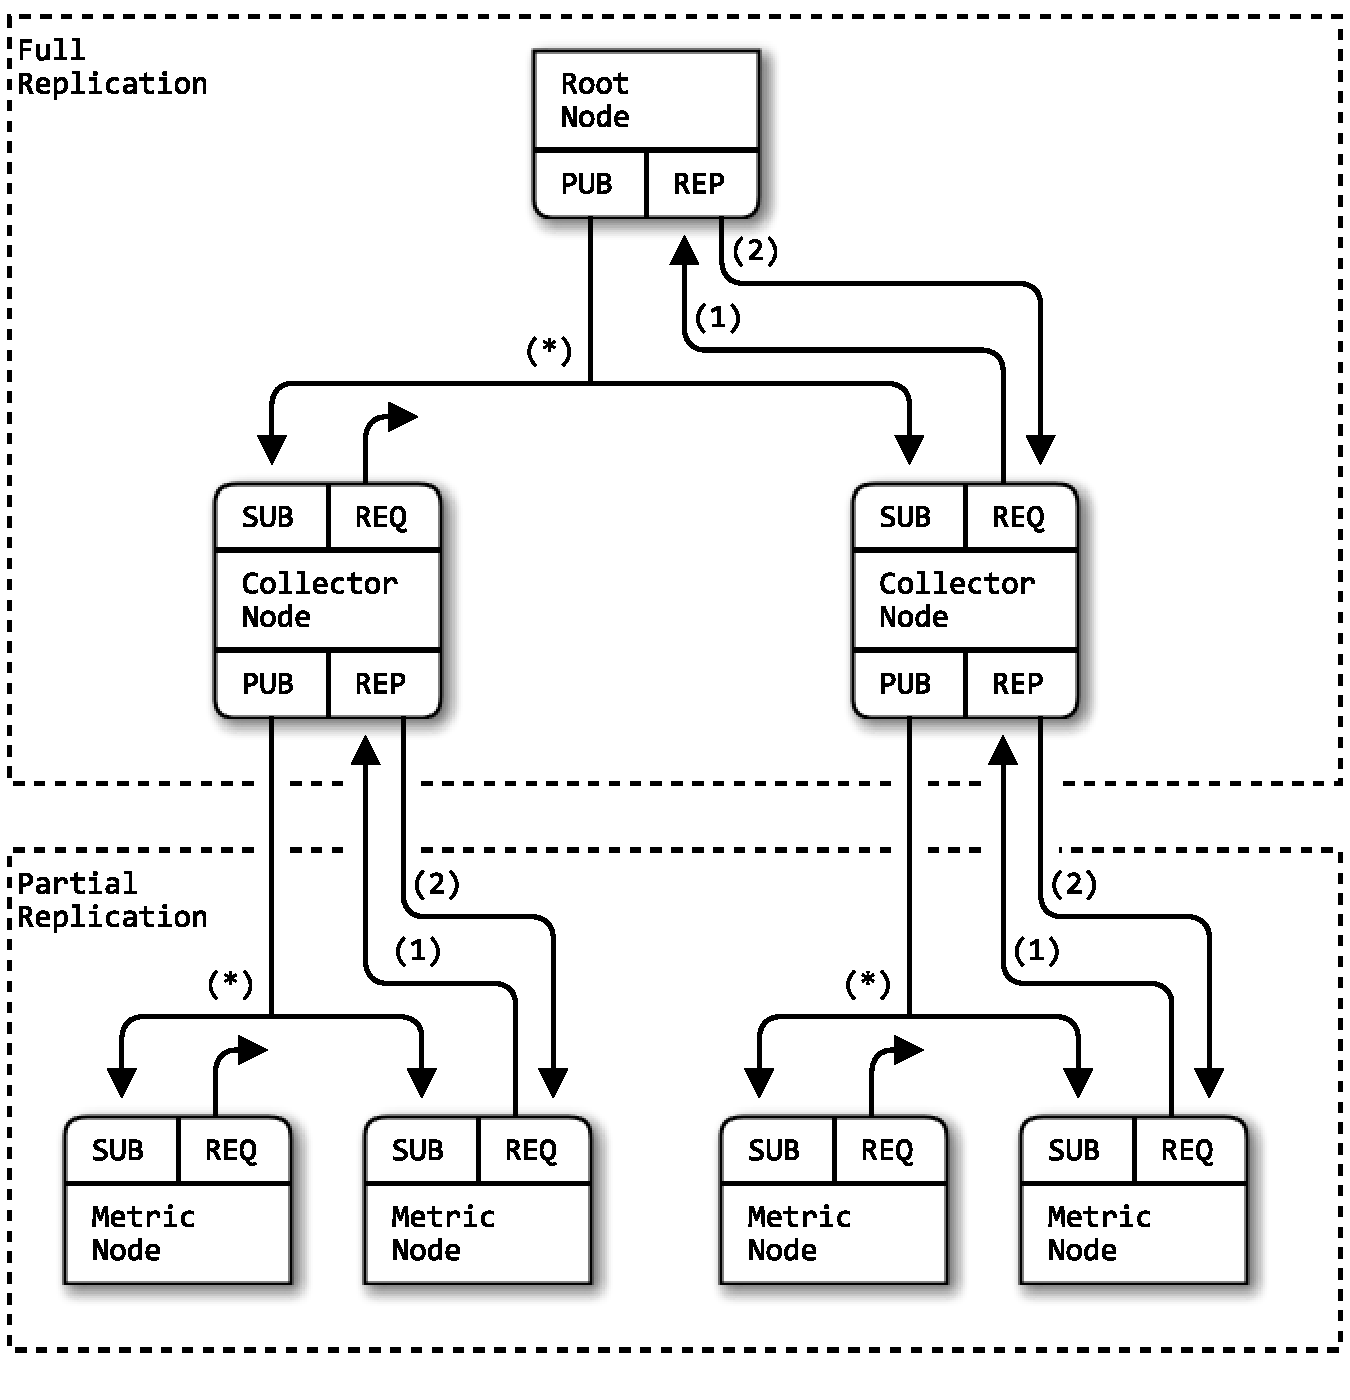
\includegraphics[height=7.6cm,transparent]{config.pdf}

\note{Notes:}
\noi{\dcamp configuration and topology state are replicated across the system using key-value pairs, with the keys laid out
in a hierarchical fashion.}
\noi{\textit{Metric} node only needs the configuration values for its particular group, the node subscribes only to the
\texttt{"/CONFIG/<group-name>/"} topic.}
\noi{Any \texttt{KVPUB} whose key does not start with this string is then discarded.}
\end{frame}

\begin{frame}[fragile,t]
\frametitle{Configuration Protocol}

The \dcamp configuration replication algorithm generally adheres to the Clustered Hashmap Protocol\cite{chp}.

\medskip

\begin{verbatim}
config-replication = *update / snap-sync
update             = P-KVPUB / P-HUGZ
snap-sync          = C-ICANHAZ ( *P-KVSYNC P-KTHXBAI )
\end{verbatim}

\note{Notes:}
\noi{A newly assigned \textbf{first-level Collector} node will first subscribe to new configuration updates from the
\textit{Root} node and then send a configuration snapshot request to the \textit{Root} node.}
\noi{A newly assigned \textbf{Metric} (or non-first-level \textit{Collector}) node will first subscribe to new
configuration updates from its parent \textit{Collector} node, and then send its parent \textit{Collector} node a
\textbf{filtered configuration snapshot request}.}
\noi{Once its snapshot has been successfully received, a node will process any pending configuration updates and then,
in the case of a \textit{Collector} node, respond to child node snapshot requests.}
\end{frame}

%------------
\begin{frame}[t]
\frametitle{Data Protocol}
There are two data flow protocols in the \dcamp system: the \textbf{external protocol} for data flowing between nodes
and the \textbf{internal protocol} for data flowing between components within a single node.

\bigskip
\centering
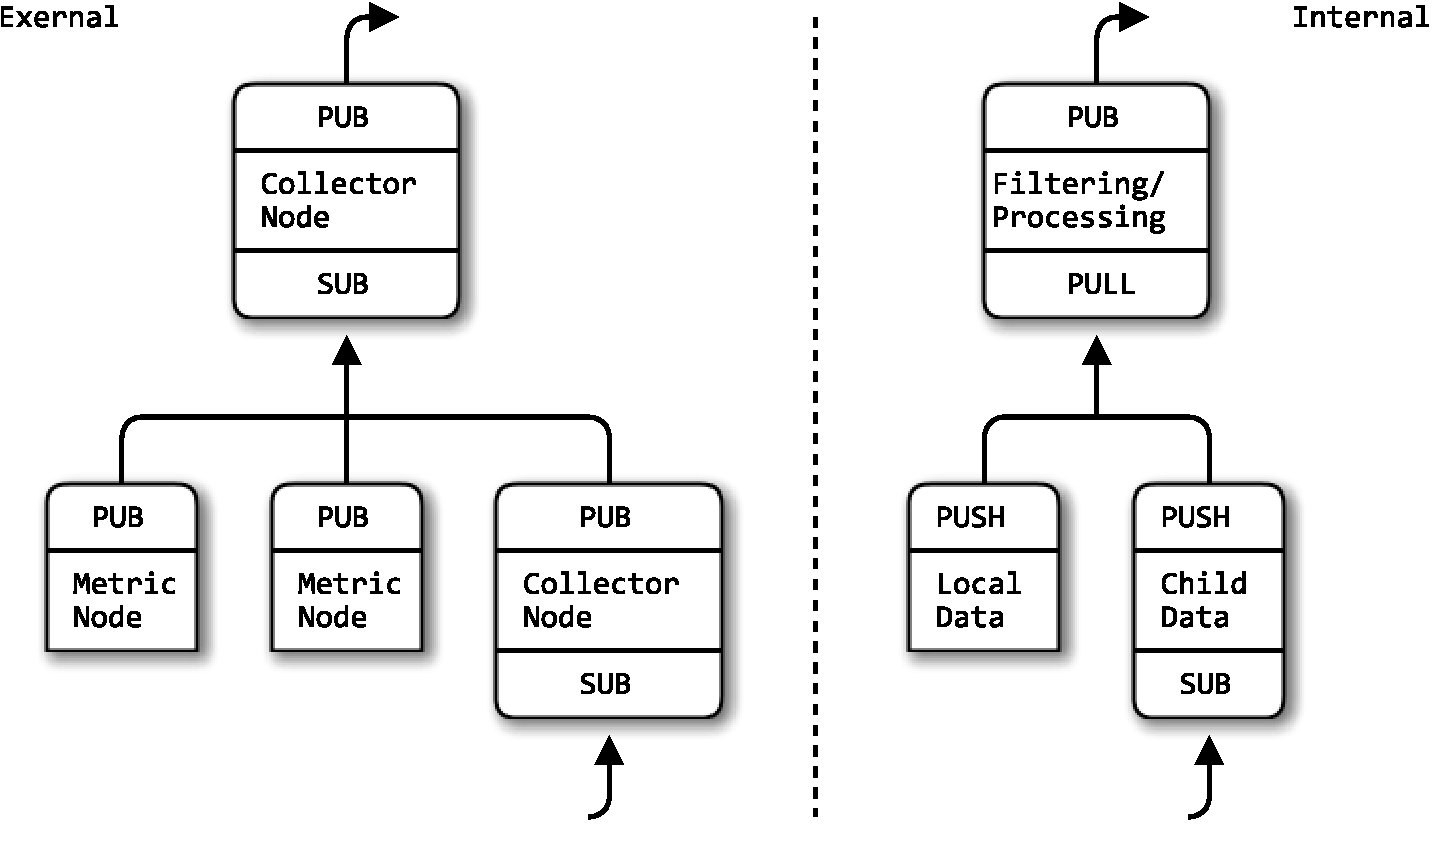
\includegraphics[scale=0.35]{data.pdf}

\note{Notes:}
\noi{Both protocols have the same specification and use the same message formats.}
\noi{The \dcamp data flow protocol is very simple: single message type.}
\noi{The data flows from one node to another via PUB/SUB sockets.}
\noi{Internally, data flows from the upstream data producers, through a filtering/processing unit, and out to downstream
data consumers via PUSH/PULL sockets.}
\noi{When data rate is slower than a predefined threshold, heartbeats are sent instead to keep inter-node connections
alive.}
\end{frame}

%------------
\begin{frame}[t]
\frametitle{Recovery Protocols: Promotion}
The \dcamp Recovery Protocols are used for the Promotion and Election algorithms and use the same base messages as the
Topology Protocol.

\bigskip
\centering
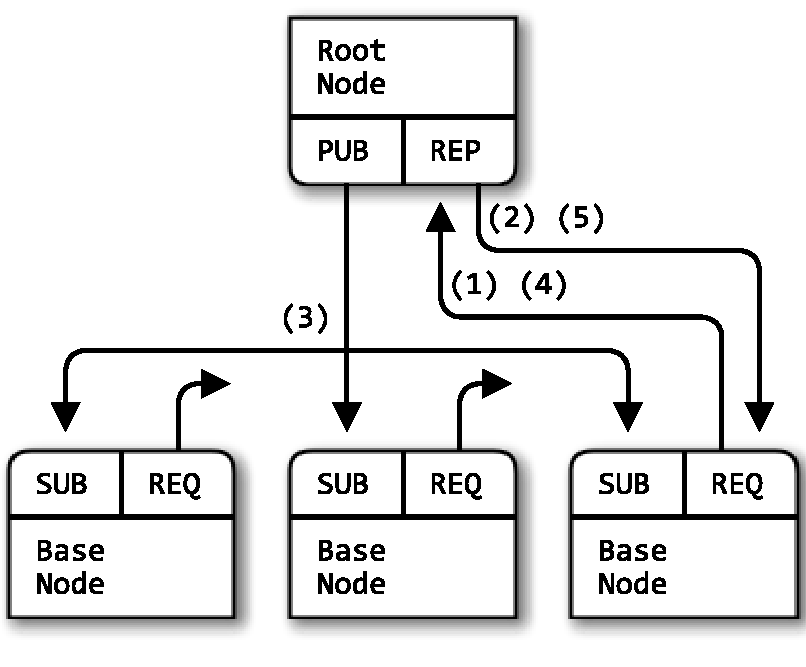
\includegraphics[scale=0.35]{branch-recovery.pdf}

\note{Notes:}
\noi{The Branch Recovery Protocol is initiated by \textit{Metric} nodes when they detect their \textit{Collector} has
died.}
\noi{Once the \textit{Root} node has received an \texttt{SOS} message from at least one third of the branch's
\textit{Metric} nodes, the \textit{Root} proceeds to shutdown the entire branch using the ``stop'' Topology Protocol.}
\noi{Once shut down, a new \textit{Collector} is selected and the branch is rebuilt using the standard ``discover''
Topology Protocol.}
\end{frame}

%------------
\begin{frame}[t]
\frametitle{Recovery Protocols: Election}
The \dcamp Recovery Protocols are used for the Promotion and Election algorithms and use the same base messages as the
Topology Protocol.

\bigskip
\centering
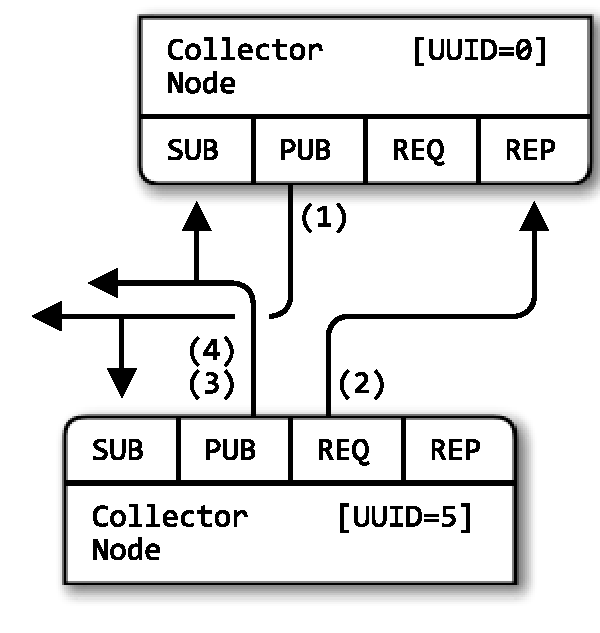
\includegraphics[scale=0.35]{root-recovery.pdf}

\note{Notes:}
\noi{As each \textit{Collector} node detects the \textit{Root} node has died, it attempts to start an election via the
\texttt{WUTUP} message.}
\noi{\textit{Collector} nodes with higher UUIDs will respond to the first \textit{Collector} by sending the \texttt{YO}
message.}
\noi{If no \texttt{YO} messages are received by the first \textit{Collector}, the \texttt{IWIN} message is sent out to
all \textit{Collector} nodes, self-declaring the first \textit{Collector} as the new Root.}
\end{frame}

%------------------------------------------------
\section{dCAMP Analysis}
%------------------------------------------------

%------------------------------------------------
\subsection{Transparency}

%------------
\begin{frame}
\frametitle{Strategy}
To measure the impact of \dcamp on a monitored process, a workload is defined and measured with and without \dcamp
active. The measured difference in performance of the monitored process is defined to be \dcampns's monitoring overhead.

\note{Notes:}
\end{frame}

%------------
\begin{frame}
\frametitle{Workload}
\textbf{Client:} Apache JMeter (v2.11) on a MacBook Pro (2.7GHz Core i7, 8GB 1333MHz DDR3, SSD) running OSX 10.9. \\
\textbf{Server:} default-configured Apache instance on a Lenovo Thinkpad (dual 2.16GHz Centrino Duo T2600, 2GB 667MHz
DDR2, SATA) running Ubuntu 13.10.

\medskip

Each test run includes 18 different load points, scaling the number of client threads from 2 to 2048. For every load
point, the threads continuously (in this order):

\begin{enumerate}
\item load a static home page,
\item load a PHP page which calculates the 25th Fibonacci number, and
\item download a 5MB file of random binary data.
\end{enumerate}

\note{Notes:}
\noi{The client machine is directly connected to the Apache server via crossover gigabit Ethernet.}
\noi{Fibonacci workload is CPU-bound, 5MB download is disk-bound, home page workload is only used to seed the client
     connection and is not part of the analysis measurements.}
\noi{After the ramp up phase of each load point (launching 10 threads per second), the test ensures all threads continue
     to execute simultaneously for five minutes before shutting down.}
\noi{The arithmetic mean of the request latency for each step at each load point is then calculated and averaged across
     three distinct runs of the same test.}
\end{frame}

%------------
\begin{frame}
\frametitle{Configuration}

Each \dcamp configuration level monitors \textbf{four global metrics} and \textbf{three process-specific metrics} on the
Apache process(es). The global metrics are CPU usage (\texttt{proc}), memory usage (\texttt{mem}), disk throughput
(\texttt{disk}), and network throughput (\texttt{net}); the Apache metrics are CPU usage (\texttt{apache\_cpu}), memory
usage (\texttt{apache\_mem}), and combined disk/network throughput (\texttt{apache\_io}).

\begin{itemize}
\item \textbf{baseline} -- \dcamp off
\item \textbf{5m} -- all metrics every 300 seconds, heartbeats every 60 seconds
\item \textbf{1m} -- all metrics every 60 seconds, heartbeats every 60 seconds
\item \textbf{10s} -- global metrics every 300 seconds, Apache metrics every 10 seconds, heartbeats every 300 seconds
\item \textbf{1s} -- global metrics every 300 seconds, Apache metrics every 1 second, heartbeats every 300 seconds
\end{itemize}

\note{Notes:}
\noi{No thresholds were defined for any of the configurations. That is, Sensor nodes immediately reported every sample
     instead of holding them for later reporting.}
\end{frame}

%------------
\begin{frame}
\frametitle{CPU-Bound Results}
\centering
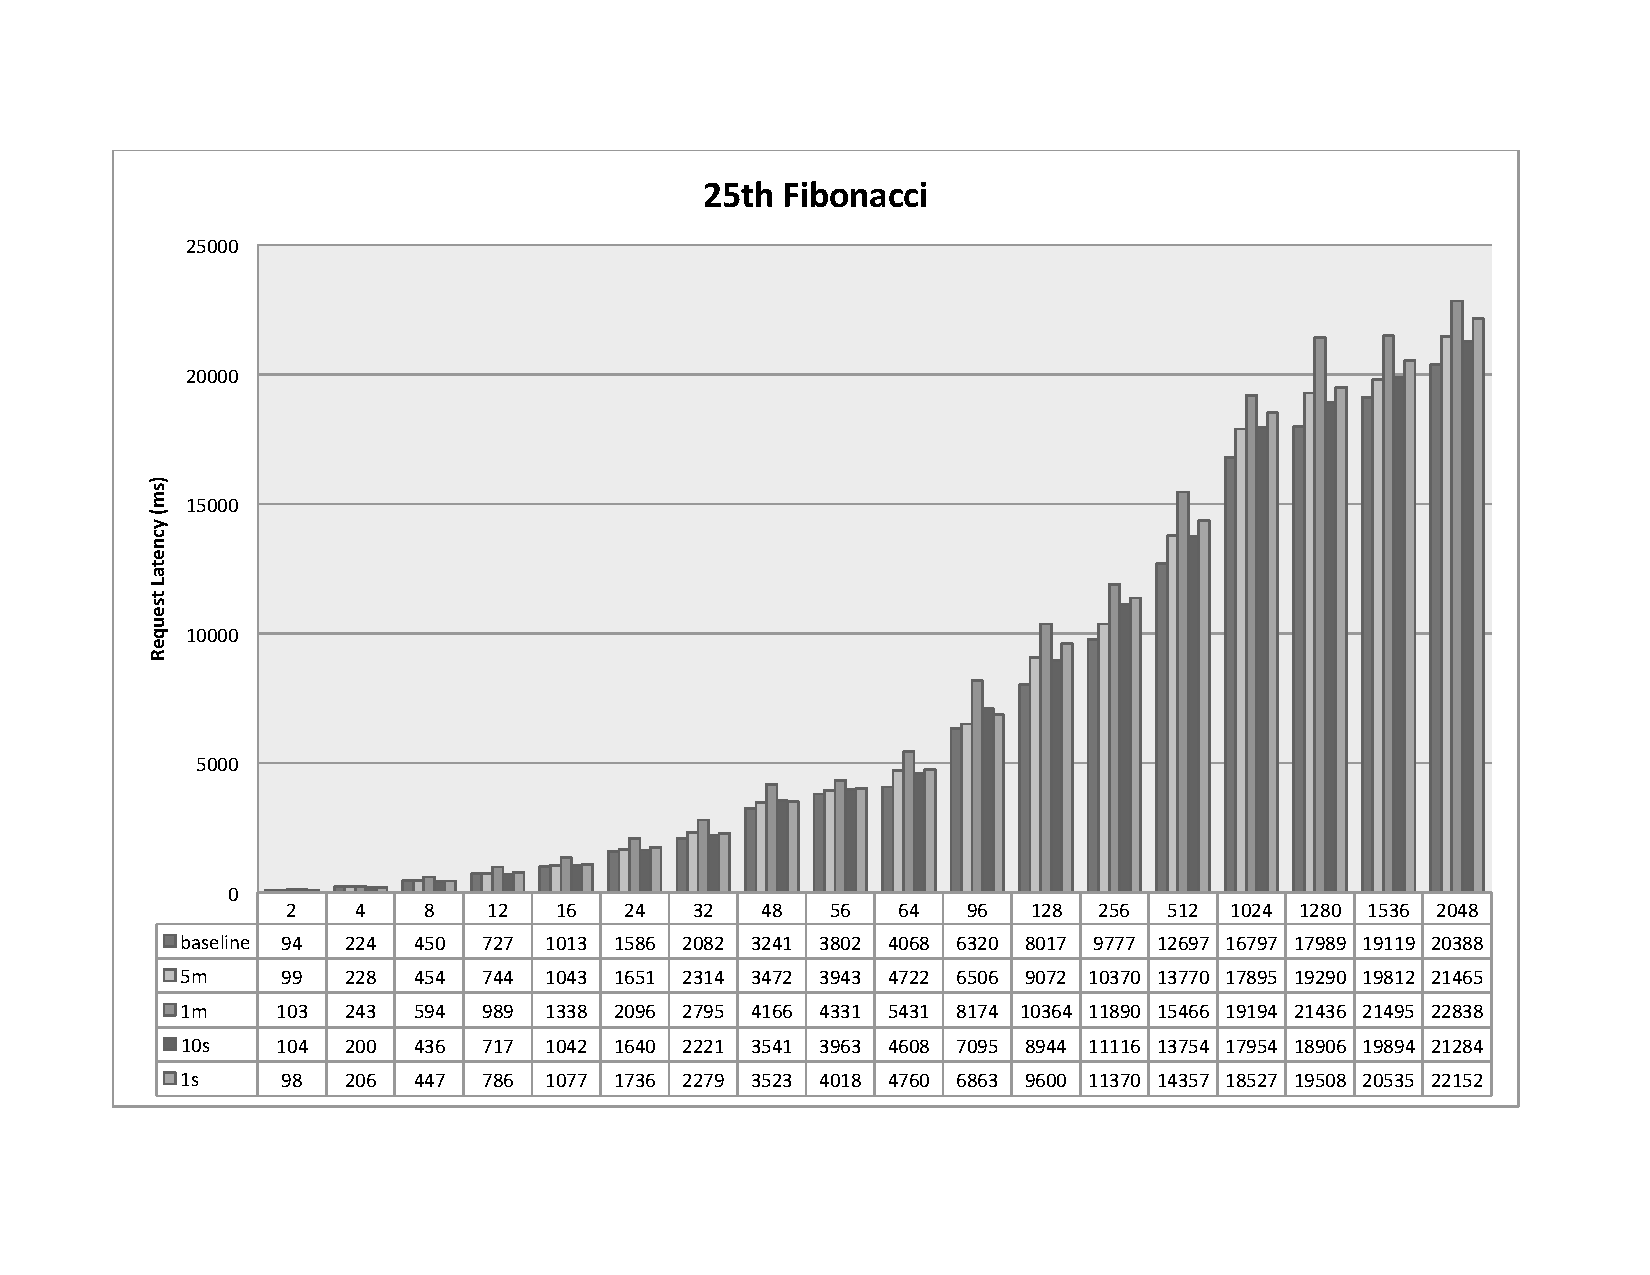
\includegraphics[height=8.6cm,transparent]{compare-fib.pdf}

\note{Notes:}
\noi{In the CPU-bound Fibonacci test, the biggest relative increase in request latency occurs between the runs with two and
four threads. This correlates to the two physical CPU cores on the system exceeding capacity.}
\noi{The 1m config run exhibits the worst performance of all the CPU-bound tests. This shows that global metric monitoring is actually more CPU
intensive than collecting per-process metrics, even for processes with many active processes.}
\noi{The rate at which request latency worsens begins to level off starting at the 512 thread load point. This is also the
load point at which Apache begins to return errors. As the percentage of requests resulting in errors increases, the
latency of the successful requests improves slightly. This explains the trend line shift.}
\end{frame}

%------------
\begin{frame}
\frametitle{Disk-Bound Results}
\centering
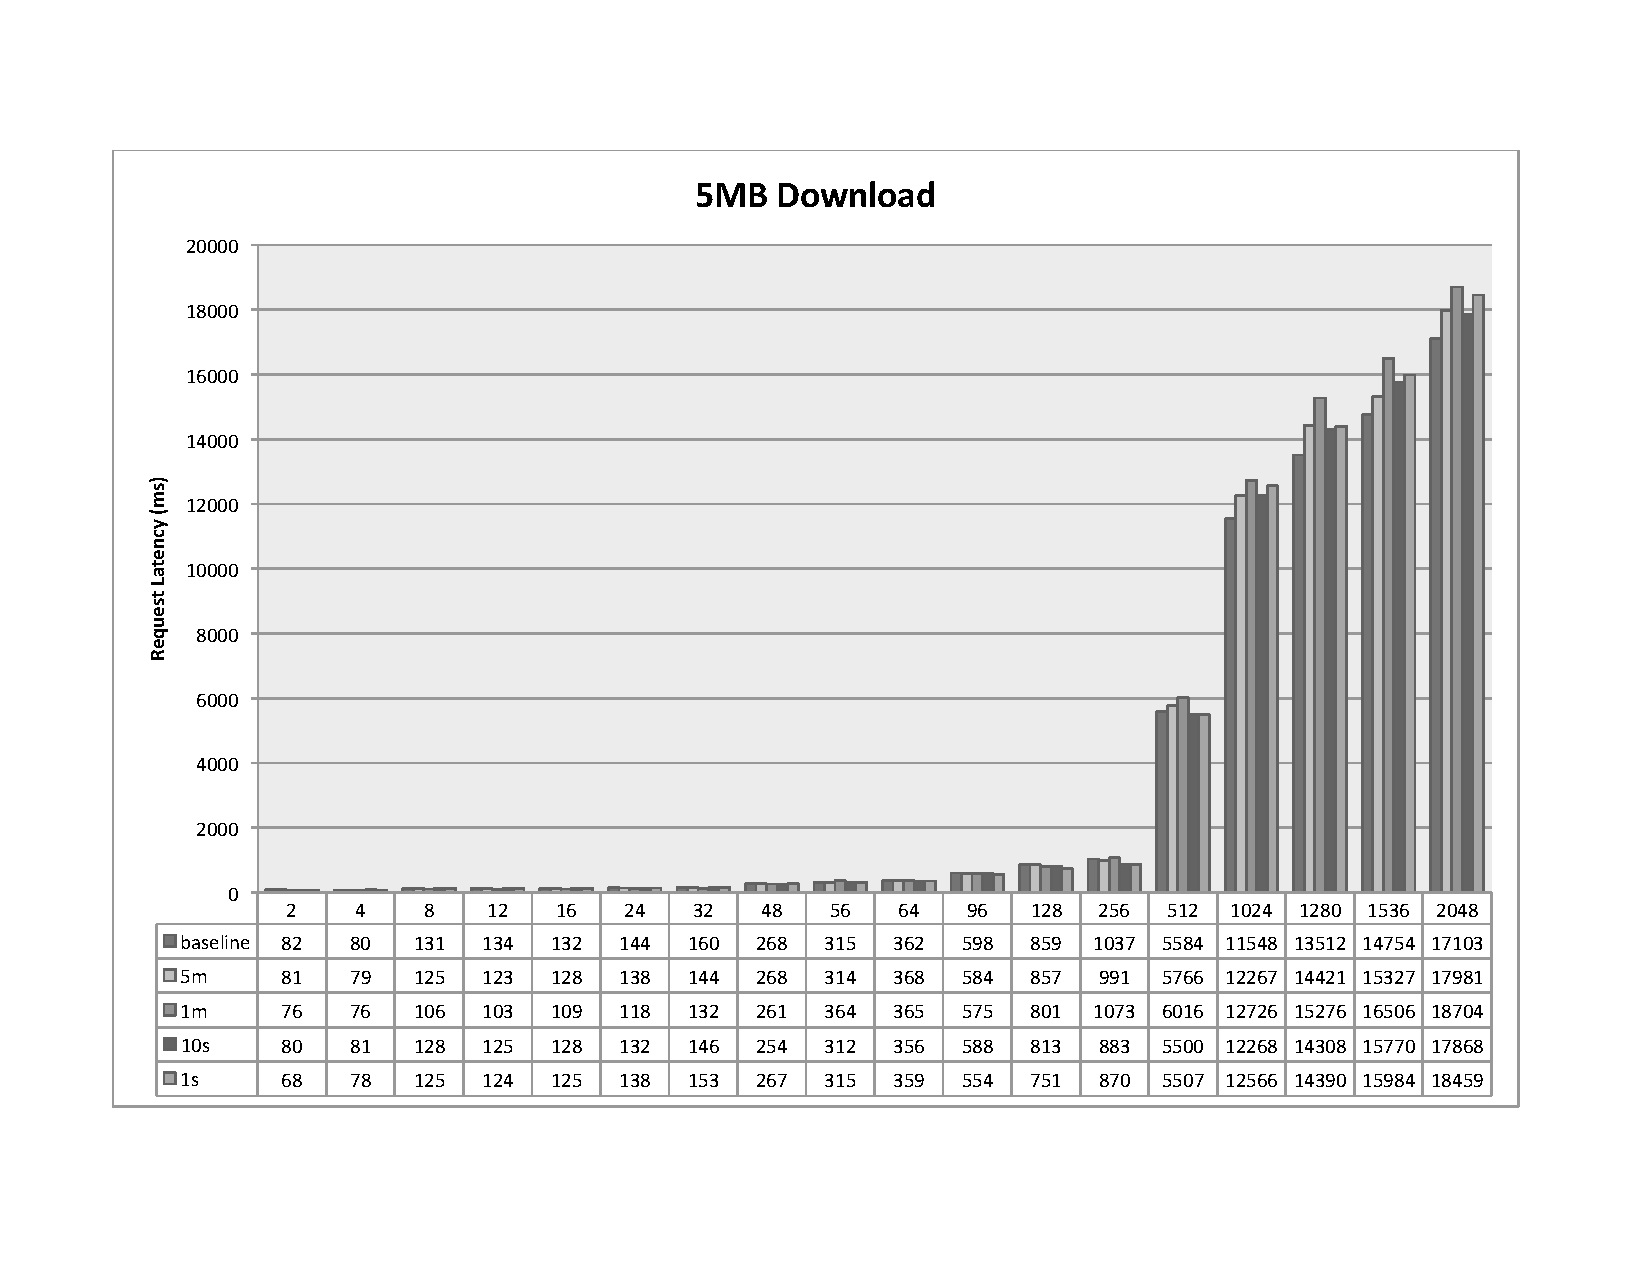
\includegraphics[height=8.6cm,transparent]{compare-down.pdf}

\note{Notes:}
\noi{Apache's disk-bound performance measured in the 5MB download test is relatively unaffected by \dcampns. This is expected
since the infrequent samples being logged to an output file are \dcampns's only disk access.}
\noi{The graph also shows the 512 thread load point as the beginning of a trend line shift, again correlating with the
increase in request error rate.}
\end{frame}

\begin{frame}
\frametitle{Observations}

\bee[<+->]
\item When nodes are not expected to fail frequently, using longer heartbeat periods reduces the impact \dcamp has on the
system.
\item It is better to monitor a process using a faster sample period than an entire system using a slower sample
period.
\item The \dcamp system impact is noticeable but a considerably smaller factor than the impact hardware limitations
have on performance monitoring.
\item Holding all else constant, slower sample periods have an obviously lower impact on system performance compared
to faster sample periods.
\item Possibly using \dcampns's reporting threshold, system impact can be minimized while still
maintaining fine sample granularity.
\eee

\note{Notes:}
\end{frame}

%------------------------------------------------
\subsection{Scalability}

%------------
\begin{frame}
\frametitle{Strategy}
One of the primary measures of scalability for a distributed system is its network traffic.\cite{zanikolas2005} By
simulating successively larger \dcamp systems (with respect to node count), one can extrapolate \dcampns's effectiveness
at monitoring large distributed systems and how to best configure its metric collections.

\note{Notes:}
\end{frame}

%------------
\begin{frame}
\frametitle{Workload}
\dcamp is setup to monitor a machine's global metrics, scaling the number of \textbf{simulated nodes in the \dcamp
system from 3 nodes up to 200 nodes}. The metric configuration is kept constant for each test run. As \dcamp starts,
monitors in steady state, and shuts down, the machine's network traffic is monitored and recorded every five seconds.

\medskip

The test machine is a MacBook Pro (2.7GHz Core i7, 8GB 1333MHz DDR3, SSD) running OSX 10.9. All simulated \dcamp nodes
use endpoints on the machine's loopback interface, and only the loopback interface traffic is monitored. The machine is
otherwise entirely idle during the test runs.

\note{Notes:}
\noi{three-node system: one \textit{Root}, one \textit{Collector}, one \textit{Metric}}
\noi{200-node system: eight groups with twenty-five nodes per group}
\end{frame}

%------------
\begin{frame}
\frametitle{Configuration}
\dcamp is configured to monitor and report the below \textbf{global metrics}, using a heartbeat of 60 seconds.

\begin{itemize}
\item CPU usage every 60 seconds
\item total disk throughput every 120 seconds
\item total network throughput every 120 seconds
\item memory usage every 60 seconds
\end{itemize}

\note{Notes:}
\noi{No thresholds were defined for the above configuration. That is, Sensor nodes immediately reported every sample instead
of holding them for later reporting.}
\end{frame}

%------------
\begin{frame}
\frametitle{Steady State Network Bytes}
\centering
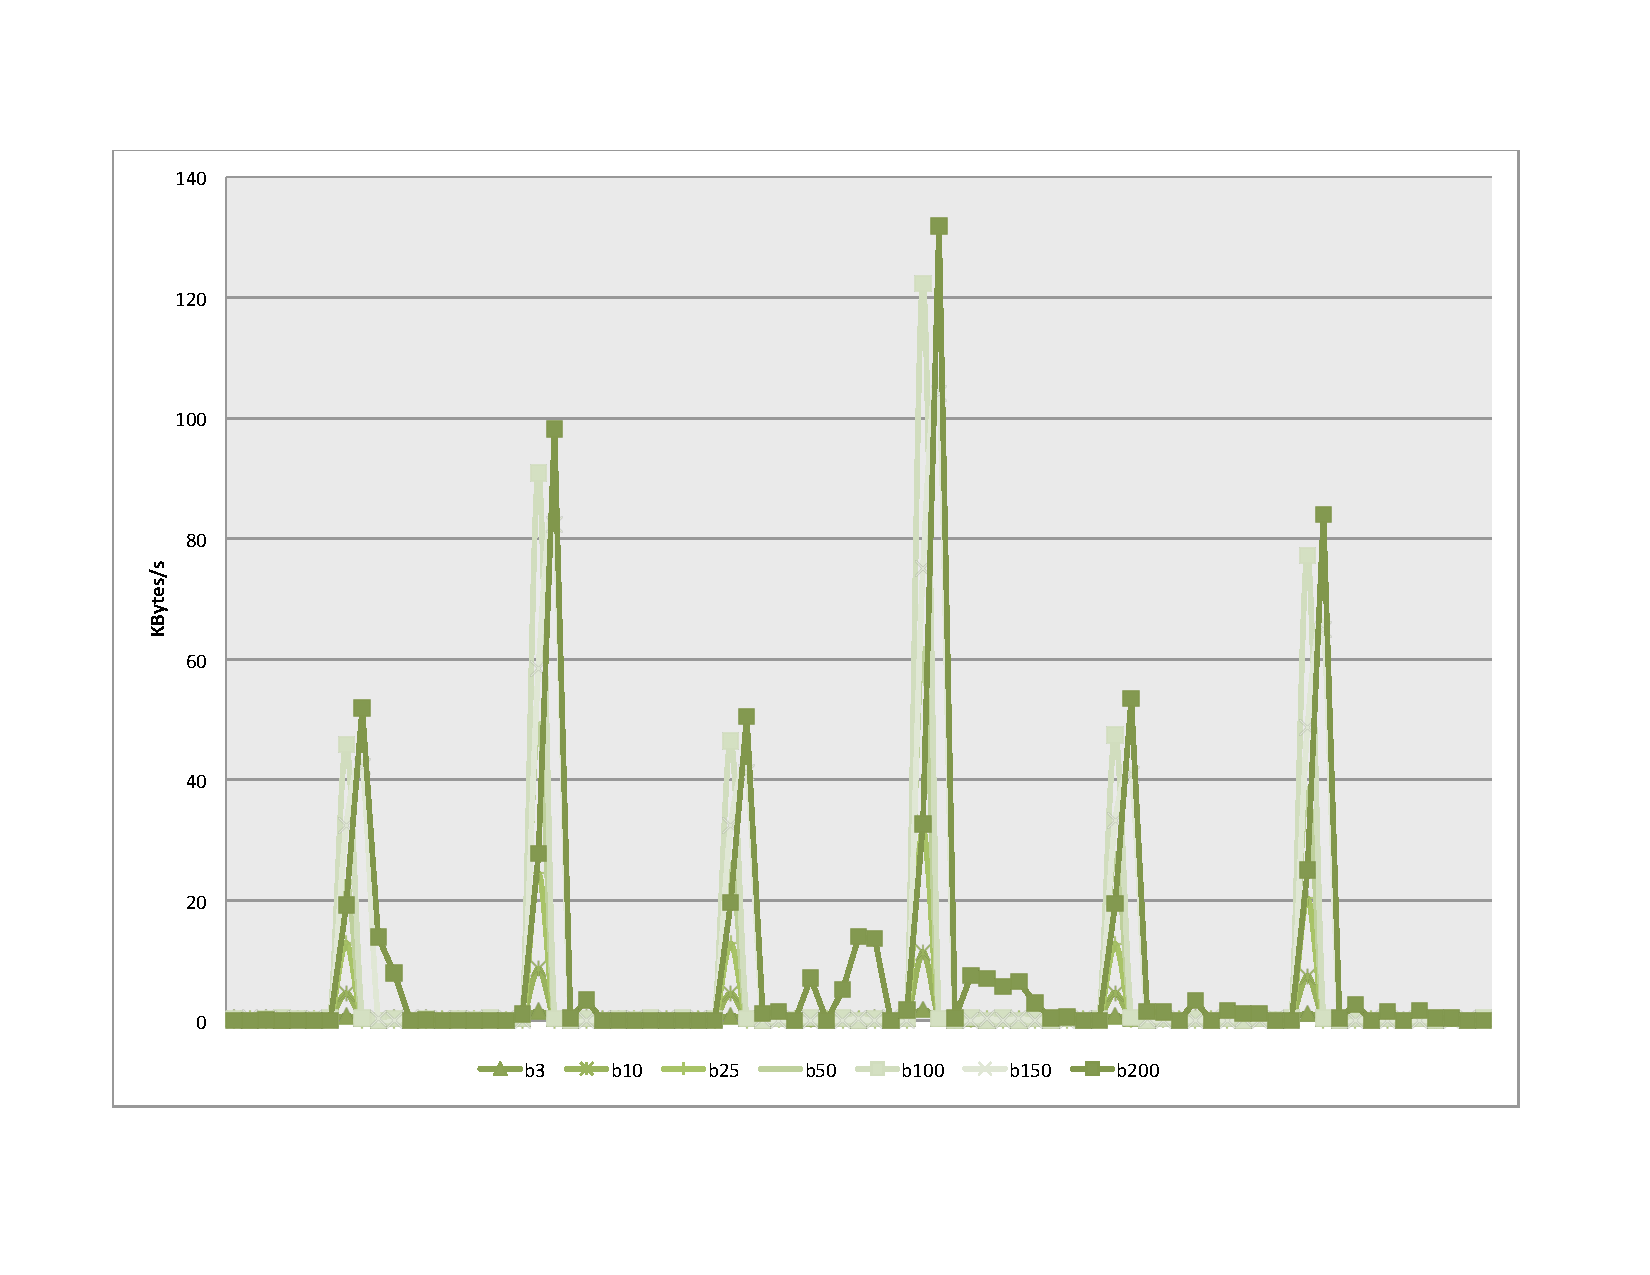
\includegraphics[height=8.6cm,transparent]{dcamp-net-bytes-steady.pdf}

\note{Notes:}
\noi{The rest (other than start-up/shut-down) of steady operation shows expected low network traffic except on sample periods.}
\end{frame}

%------------
\begin{frame}
\frametitle{Steady State Network Packets}
\centering
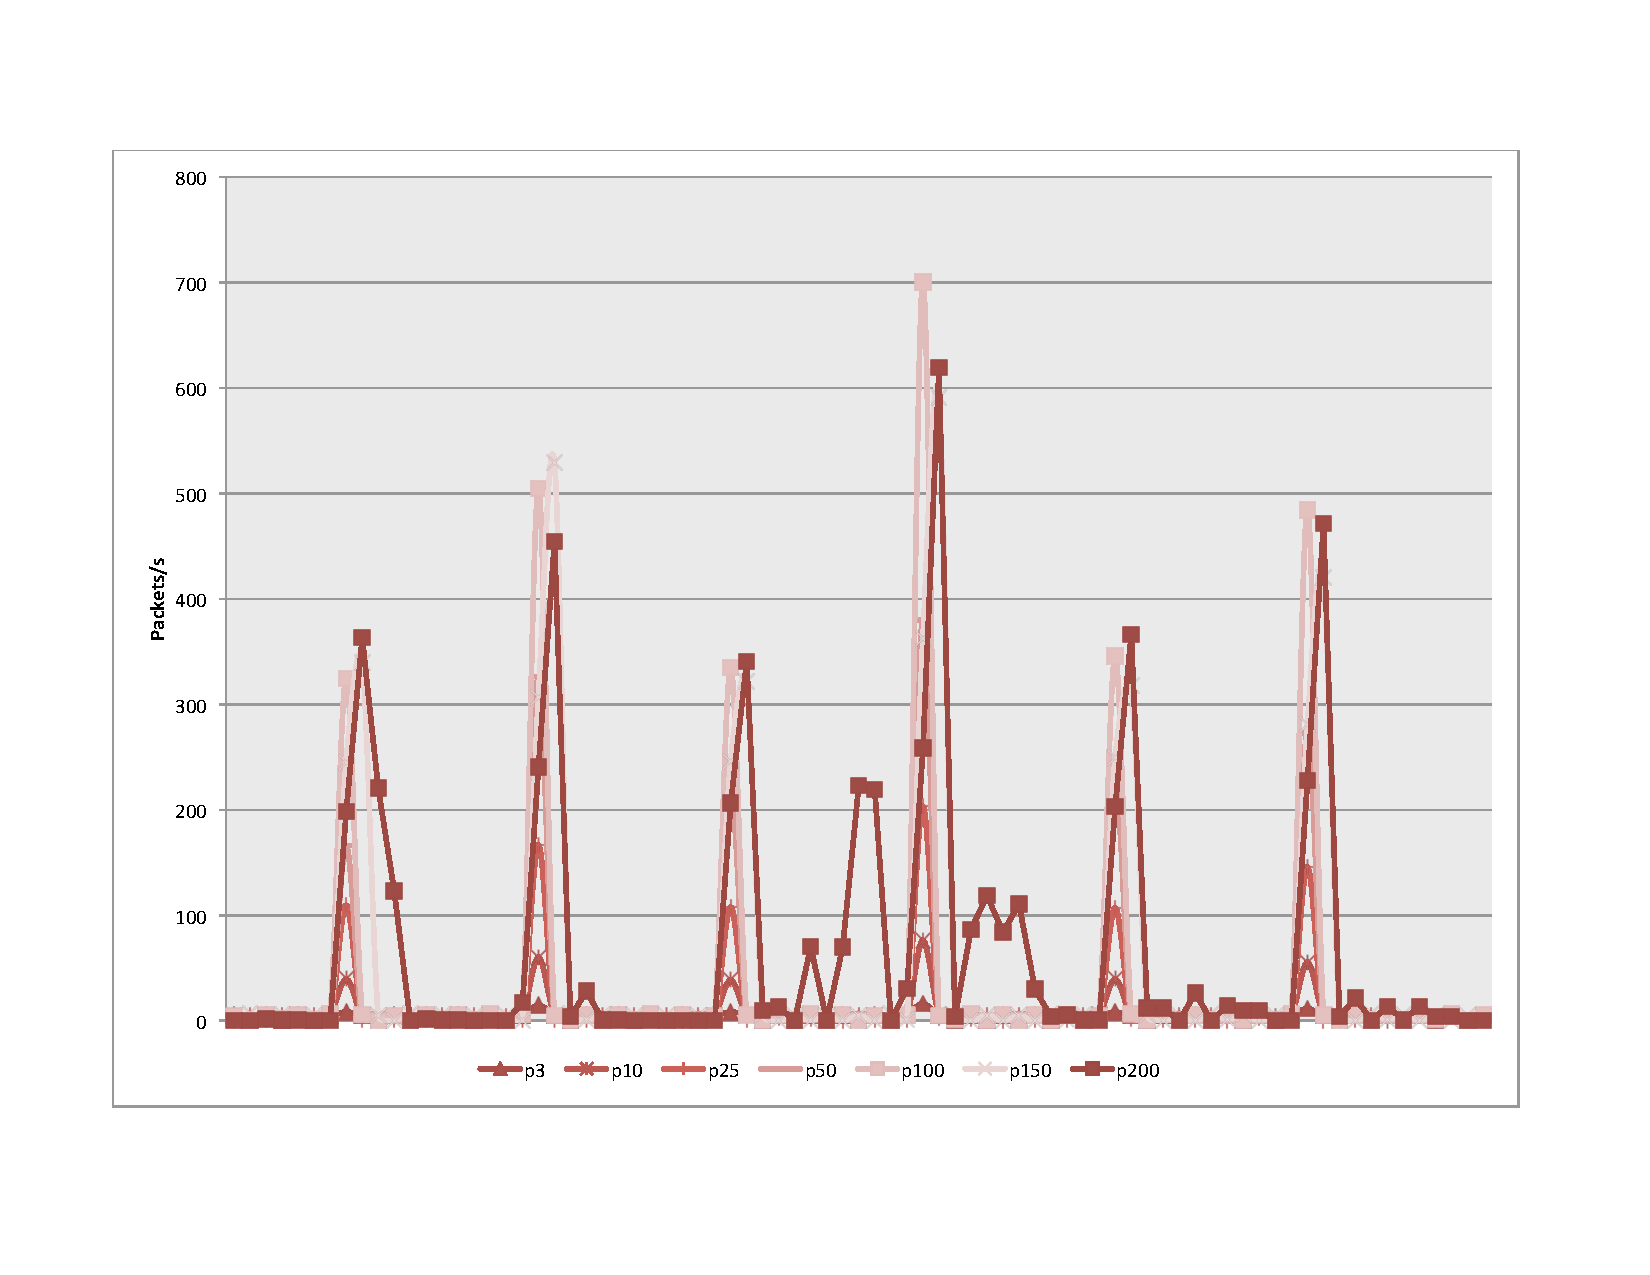
\includegraphics[height=8.6cm,transparent]{dcamp-net-packets-steady.pdf}

\note{Notes:}
\end{frame}

%------------
\begin{frame}
\frametitle{Average Network Utilization}
\centering
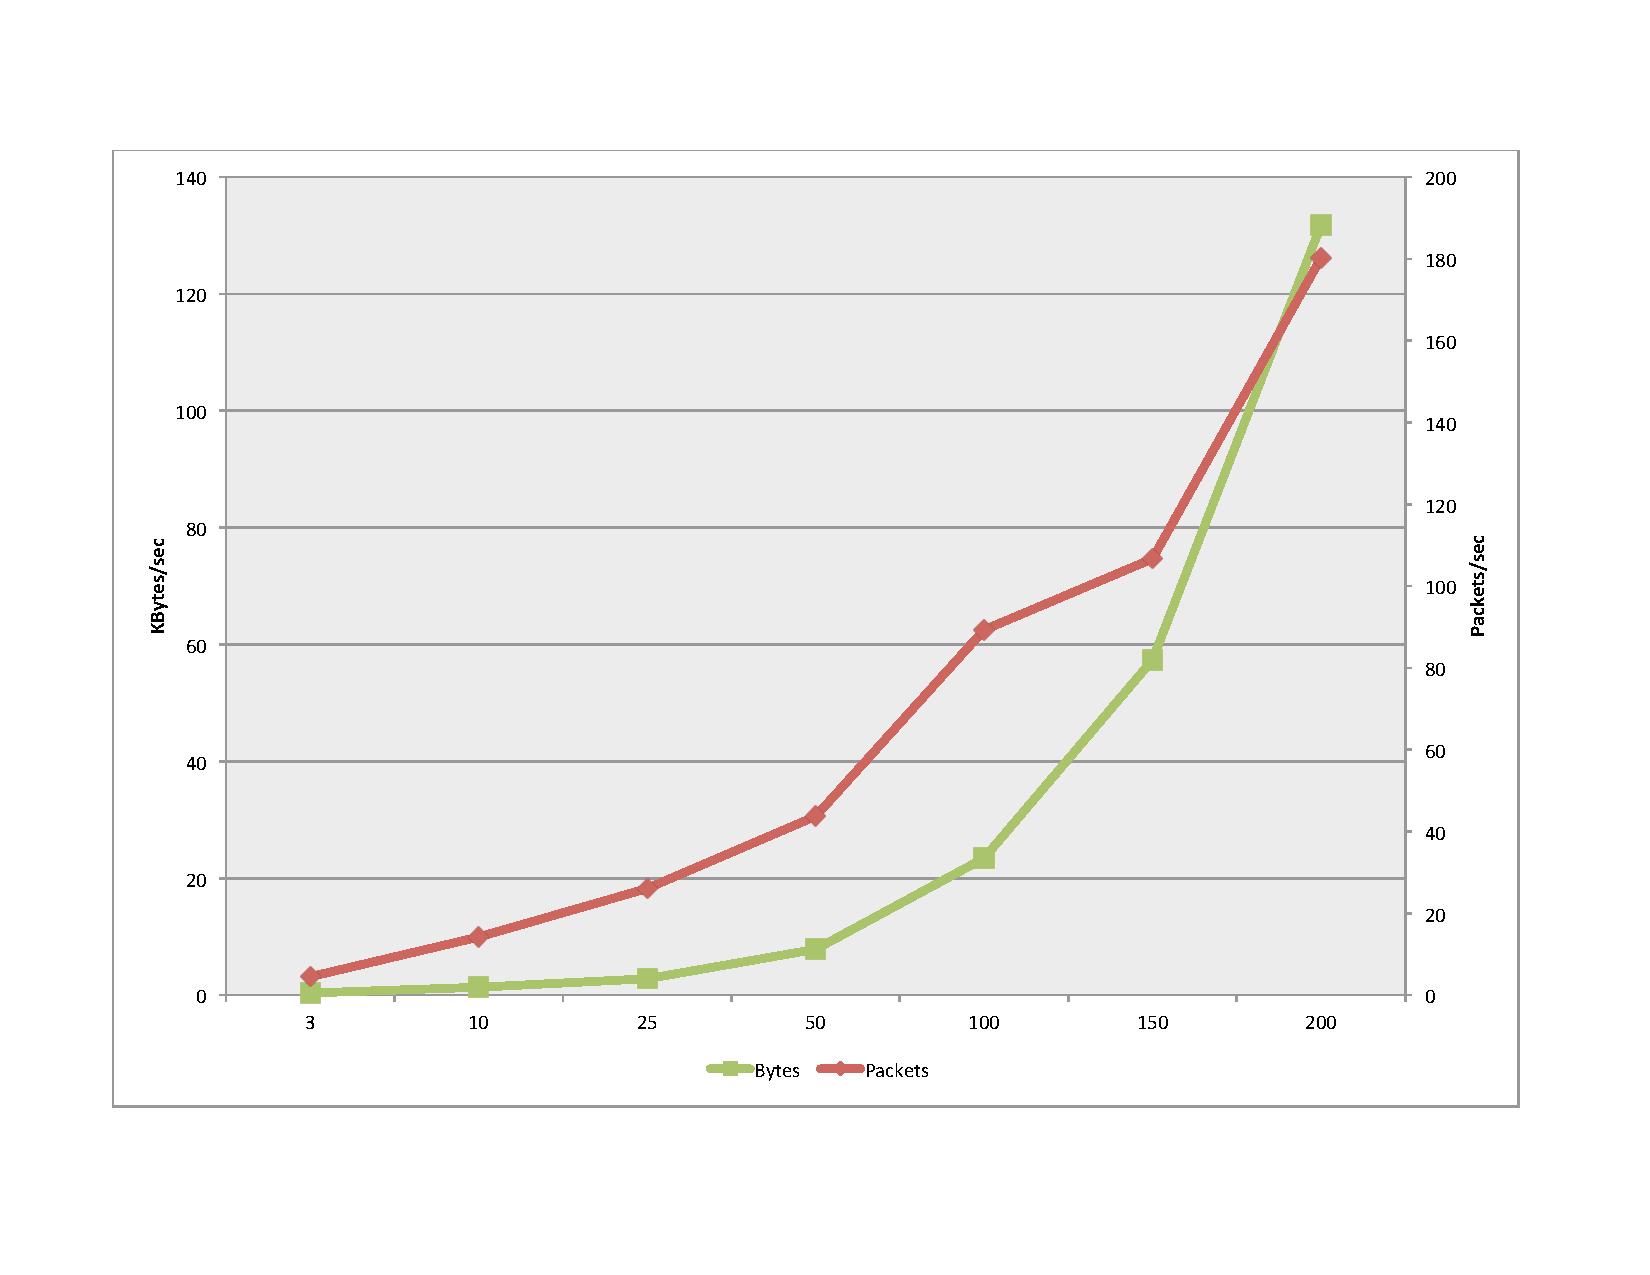
\includegraphics[height=8.6cm,transparent]{dcamp-net-average.pdf}

\note{Notes:}
\end{frame}

%------------
\begin{frame}
\frametitle{Average Network Utilization Per Node}
\centering
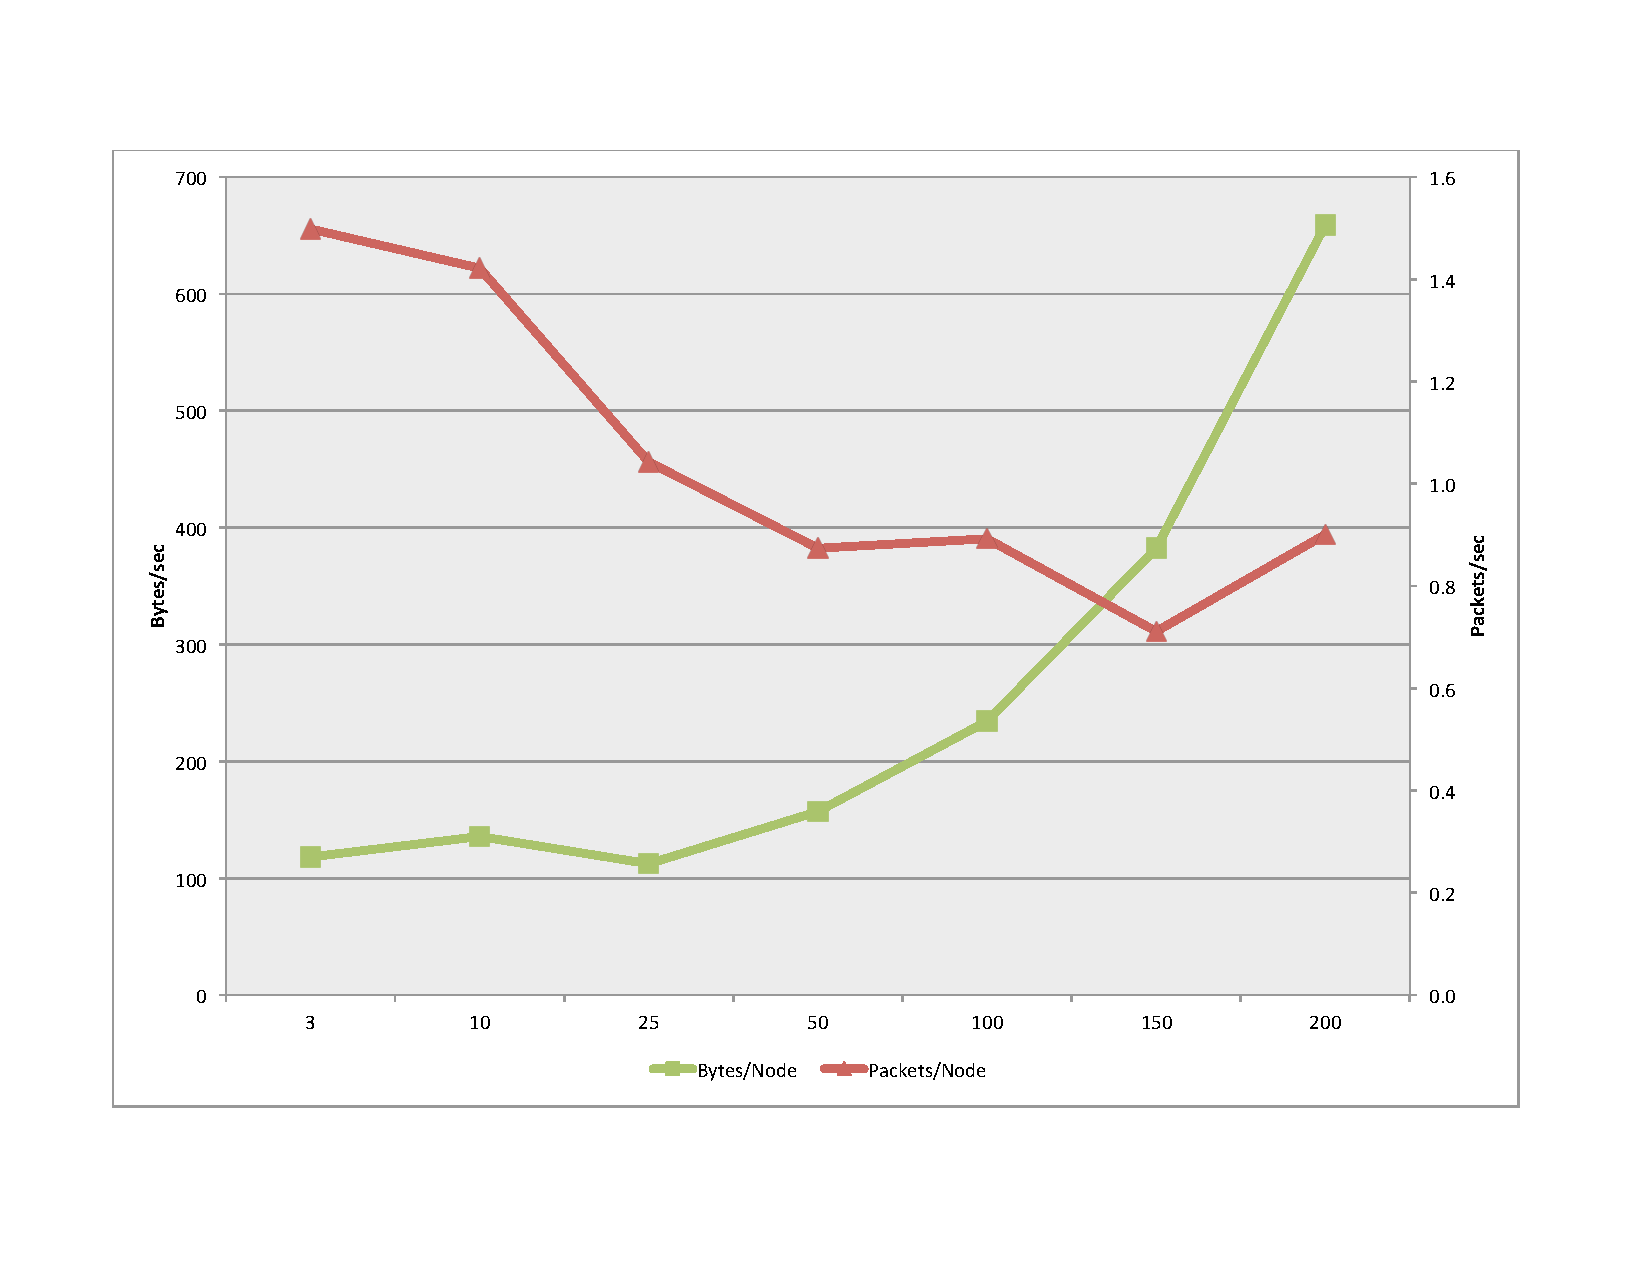
\includegraphics[height=8.6cm,transparent]{dcamp-net-average-pernode.pdf}

\note{Notes:}
\end{frame}

%------------
\begin{frame}
\frametitle{Observations}

\bee[<+->]
\item Sparklines of each load point show the same pattern: highest network traffic occurs during start up and then also
on shutdown.
\item As the node count increases, the rate at which bytes/packets are sent and received increases.
\item Comparing the same rates to the number of nodes in the system, one sees the configuration size grows faster than
the number of nodes.
\item The number of messages being sent per node actually goes down and levels off just under 1 packet per node per
second.
\item As the ratio of Sensor to Collector increases, the number of messages per node is expected to decrease. Therefore,
a higher number of child nodes per parent should result in lower network utilization and better \dcamp scalability.
\eee

\note{Notes:}
\noi{traffic at start/end: follows from \dcampns's use of chatty configuration protocols and a terse data protocol.}
\noi{node count + net increase: correlates with the larger configuration which \dcamp must track as well as the
additional nodes sending and receiving data.}
\noi{bytes per node: more configuration data to pass around}

\noi{packets per node: can be attributed to the fact that the number of Sensor nodes increases faster in relation to the
number of \textit{Collector} nodes.}
\noi{That is, Sensor nodes do not require full-configuration replication and send/receive fewer messages since they are
relatively uninvolved with topology coordination in comparison to \textit{Collector} nodes.}

\end{frame}

%------------------------------------------------
\section{Evaluation and Conclusion}
%------------------------------------------------

%------------------------------------------------
\begin{frame}
\frametitle{Evaluation}
The previous section presents an empirical evaluation of \dcampns's \textbf{transparency} and \textbf{scalability},
showing \dcamp to be both transparent and scalable when properly configured.

\medskip

\textbf{Validity} and \textbf{portability} are inherited from \camp as well as the use of portable Python libraries.
\dcampns's \textbf{data delivery models} and \textbf{completeness} are apparent in the system's design and configuration
capabilities, and these will be easily achieved with a full implementation of \dcampns.

\medskip

Likewise, updating \dcamp to meet the \textbf{security} criterion is unfinished work, but the \dcamp design and use of
ZeroMQ makes this work straightforward.

\note{Notes:}
\noi{The updated distributed performance framework criterion is introduced and used to evaluate \dcampns.}
\noi{several improvements can be made to further \dcampns's transparency and scalability}
\end{frame}

%------------------------------------------------
\begin{frame}
\frametitle{Contributions}
In this work I presented the \textbf{Distributed Common API for Measuring Performance}, a distributed performance
framework built on top of \camp \cite{gabel2007}. I described the design and implementation of \dcampns, using roles and
services on top of ZeroMQ to build a simple, reliable distributed system.

\medskip

I also presented a set of \textbf{criterion for evaluating distributed performance frameworks} by extending and updating
the criterion presented in \cite{zanikolas2005}. I used this criterion to evaluate \dcamp along with several other level
2 distributed performance frameworks and related works.

\note{Notes:}
\noi{again, level 2: dpf with at least one type of republisher in addition to producers}
\end{frame}

%------------
\begin{frame}
\frametitle{References}
\footnotesize{
\begin{thebibliography}{99} % Beamer does not support BibTeX so references must be inserted manually as below

\bibitem{gabel2007}[Gabel, 2007] {Gabel, Mark and Haungs, Michael} (2007)
\newblock {{CAMP}: a common {API} for measuring performance}
\newblock \emph{LISA'07: Proceedings of the 21st conference on Large Installation System Administration Conference}, p1--14

\bibitem{chp}[Hintjens, 2011] {Pieter Hintjens} (2011)
\newblock {Clustered Hashmap Protocol}
\newblock {\url{http://rfc.zeromq.org/spec:12/CHP}}, April 2011

\bibitem{zanikolas2005}[Zanikolas, 2005] {Zanikolas,, Serafeim and Sakellariou,, Rizos} (2005)
\newblock A taxonomy of grid monitoring systems
\newblock \emph{Future Gener. Comput. Syst.} 21(1), 0167-739X, p163--188.

\end{thebibliography}
}
\end{frame}

%----------------------------------------------------------------------------------------
%----------------------------------------------------------------------------------------

\appendix

\section{\appendixname}
\frame{\tableofcontents}

%------------------------------------------------
\subsection{Terminology}

%------------
\begin{frame}
\frametitle{Terminology}
\begin{description}

\item[\dcamp Service:]
Services are a way of logically grouping functions within the \dcamp system. Each service is implemented in \dcamp as an
independent thread.

\item[\dcamp Role:]
Roles in the \dcamp system are groupings of one or more \dcamp services. There does not exist a one-to-one
relationship between roles and services.

\item[ZeroMQ:]
ZeroMQ is a message queuing framework which allows a developer to build distributed systems by focusing on the data
and implementing simple design patterns.

\item[ZeroMQ Address:]
A \O MQ address is the combination of network host identifier (i.e. an IP Address or resolvable name) and Internet
socket port number. 

\item[ZeroMQ Endpoint:]
An endpoint is the combination of any ZeroMQ transport (\texttt{pgm}, \texttt{inproc}, \texttt{ipc}, or \texttt{tcp})
and a \O MQ address.

\end{description}
\end{frame}

%------------
\begin{frame}
\frametitle{Terminology}
\begin{description}

\item[Performance Metric:]
Performance metrics are any data about a given node relating to its throughput, capacity, utilization, or latency.

\item[Metric Sampling:]
Metric collection or sampling is the process of measuring metrics on a given node. 

\item[Metric Reporting:]
Metric reporting is the process of sending sampled metrics to a parent node.

\item[Metric Aggregation:]
Metric aggregation is the process of combining metrics from multiple nodes into a single metric, providing a coarser
granularity for the performance metrics. Metrics are combined by calculating a sum, average, percent, or any other
mathematically relevant operation.

\item[Metric Calculation:]
Metric calculation is the process of combining identical metrics from multiple timestamps into a single metric.

\end{description}
\end{frame}

%------------------------------------------------
\subsection{Evaluation Criterion Details}

%------------
\begin{frame}
\frametitle{Data Delivery Models}
Monitoring information includes fairly static (e.g., software and hardware configuration of a given node) and dynamic
events (e.g., current processor load, memory), which suggests the use of different measurement policies (e.g., periodic
or on demand). In addition, consumer patterns may vary from sparse interactions to long lived subscriptions for
receiving a constant stream of events. In this regard, the monitoring system must support both pull and push data
delivery models.
\end{frame}

%------------
\begin{frame}
\frametitle{Security}
Certain scenarios may require a monitoring service to support security services such as access control, single or mutual
authentication of parties, and secure transport of monitoring information.
\end{frame}

%------------
\begin{frame}
\frametitle{Scalability}
Monitoring systems have to cope efficiently with a growing number of resources, events and users. This scalability can
be achieved as a result of good performance which guarantees that a monitoring system will achieve the needed throughput
within an acceptable response time in a variety of load scenarios.
\end{frame}

%------------
\begin{frame}
\frametitle{Transparency}
Transparency refers to the lack of impact a distributed performance framework makes on the system being monitored. As
\cite{zanikolas2005} states, it is ``typically measured as a function of host (processor, memory, I/O) and network load
(bandwidth) generated by the collection, processing and distribution of events.'' If a framework lacks transparency it
will fail to allow the underlying distributed system to perform well and will produce inaccurate performance
measurements, thereby reducing its Scalability and destroying its Validity.
\end{frame}

%------------
\begin{frame}
\frametitle{Completeness}
The Completeness of a distributed performance framework refers to the exhaustiveness to which it gathers performance
metrics. At a minimum, a framework must provide interfaces for measuring and aggregating performance data about a
system's processor, memory, disk, and network usage. Several distributed performance frameworks provide further detailed
performance metrics about the given distributed system being monitored, but this is usually at the cost of Portability.
\end{frame}

%------------
\begin{frame}
\frametitle{Validity}
A distributed performance framework is only as good as the data is produces; if the sensors or gathering techniques are
inaccurate, then the data is useless at best, misleading at worst. Validity of a framework is achieved when the authors
of a framework provide formal verification of its accuracy.
\end{frame}

%------------
\begin{frame}
\frametitle{Portability}
A framework's ability to run on a completely heterogeneous distributed system without special considerations by the
practitioner is what this work defines as Portability. More specifically, a portable framework has a unified API
regardless of the system architecture, does not restrict itself to applications written in specific programming
languages, and does not require practitioners to manually instrument their application code. This black box
characteristic is vital for a viable distributed performance framework's effectiveness as it allows practitioners to
focus on the performance data and not on a myriad of APIs for various architectures or languages.
\end{frame}

%------------------------------------------------
\subsection{Related Work}

%------------
\begin{frame}
\frametitle{NetLogger}
Their research has shown NetLogger to be highly scalable, complete, and transparent as well as valid. The activation
service provides a push data delivery and can utilize the security mechanisms part of current web services in order to
authenticate requests for performance data. NetLogger is currently implemented for C, C++, Java, Perl, and Python
applications. Because the framework lacks black box characteristics, its \textbf{portability is greatly reduced}.
\end{frame}

%------------
\begin{frame}
\frametitle{JAMM}
JAMM, being heavily based off of NetLogger, inherits the validity, completeness, security, and transparency of NetLogger
along with its lack of \textbf{portability}. JAMM does, however, prove itself in terms of scalability with it's own
architecture.
\end{frame}

%------------
\begin{frame}
\frametitle{Hawkeye}
While no experiments have been run, the generally centralized manager reduces the Hawkeye framework's scalability, and
its transparency is unknown. The frameworks module based producer architecture gives it an infinite completeness, but
being only available on Linux and Solaris makes the framework less \textbf{portable}. Lastly, the ability to run jobs
\textbf{securely} on target machines has been left as future work by the authors.
\end{frame}

%------------
\begin{frame}
\frametitle{SCALEA-G}
The framework makes use of secure sockets to achieve secure communications and achieves high completeness via code
instrumentation. Unfortunately, the authors do not provide any report on SCALEA-G's \textbf{validity} or
\textbf{transparency}.
\end{frame}

%------------
\begin{frame}
\frametitle{SCALEA-G}
The framework makes use of secure sockets to achieve secure communications and achieves high completeness via code
instrumentation. Unfortunately, the authors do not provide any report on SCALEA-G's \textbf{validity} or
\textbf{transparency}.
\end{frame}

%------------
\begin{frame}
\frametitle{Host sFlow}
In supporting host and application performance metric analysis alongside network metrics in one common system, sFlow has
an advantage over more traditional host-only distributed performance frameworks. While sFlow's claims to scalable and
accurate network level monitoring have been validated, less work has been to show the same for Host sFlow.
\end{frame}

%------------
\begin{frame}
\frametitle{Ganglia}
The analysis presented shows the design scales and maintains transparency for systems of several hundred nodes. Still,
\textbf{scalability} is a concern of the authors since the multicast protocol exhibits a quadratic trendline as the
number of nodes within a cluster increases. Memory usage and inter-cluster bandwidth also increase as the number of
nodes increases, albeit much more linearly. In comparison, \dcamp memory usage is nearly constant since performance data
is not persisted in memory to the same extent.
\end{frame}

%------------------------------------------------
\subsection{ZeroMQ: Sockets and Patterns}

%------------
\begin{frame}
\frametitle{ZeroMQ in 100 Words}
\begin{quote}
\O MQ (also known as ZeroMQ, 0MQ, or zmq) looks like an embeddable networking library but acts like a concurrency
framework. It gives you sockets that carry atomic messages across various transports like in-process, inter-process,
TCP, and multicast. You can connect sockets N-to-N with patterns like fan-out, pub-sub, task distribution, and
request-reply. It's fast enough to be the fabric for clustered products. Its asynchronous I/O model gives you scalable
multicore applications, built as asynchronous message-processing tasks. It has a score of language APIs and runs on most
operating systems. \O MQ is from iMatix [\url{http://www.imatix.com}] and is LGPLv3 open source.
\end{quote}
\end{frame}

%------------
\begin{frame}
\frametitle{ZeroMQ Sockets}
\O MQ sockets mimic standard TCP sockets, exposing interfaces for creating and destroying instances, binding and
connecting to network endpoints, and sending and receiving data. However, they have two key differences from their
TCP counterparts.

\bei
\item asynchronous---the actual sending and receiving of data on a ZeroMQ socket is handled by a background thread.
\item built-in support for one-to-many connections; a single socket can send and receive data from multiple endpoints.
\eei
\end{frame}

%------------
\begin{frame}
\frametitle{ZeroMQ Messages}
ZeroMQ messages are the building blocks of all data sent across ZeroMQ sockets. A message is comprised of one or more
frames (or parts), and a single frame can be any size (including zero) that fits in memory. ZeroMQ guarantees messages
are delivered atomically, meaning either all frames of the message are sent/received or none of the frames. Lastly,
because sockets are asynchronous and messages are atomic, the entire message must fit in memory.
\end{frame}

%------------
\begin{frame}
\frametitle{ZeroMQ Messaging Patterns}
\begin{description}

\item[Publish-Subscribe:]
``The publish-subscribe pattern is used for one-to-many distribution of data from a single publisher to multiple
subscribers in a fan out fashion.''

\item[Request-Reply:]
``The request-reply pattern is used for sending requests from a [...] client to one or more [...] services, and receiving
subsequent replies to each request sent.''

\item[Pipeline:]
``The pipeline pattern is used for distributing data to nodes arranged in a pipeline. Data always flows down the
pipeline, and each stage of the pipeline is connected to at least one node. When a pipeline stage is connected to
multiple nodes data is round-robined among all connected nodes.''

\item[Exclusive Pair:]
``The exclusive pair pattern is used to connect a peer to precisely one other peer. This pattern is used for inter-thread
communication across the inproc transport.''
\end{description}
\end{frame}

%------------------------------------------------
\subsection{dCAMP Metrics}

%------------
\begin{frame}
\frametitle{Metric Groups}
In \dcampns, metrics are grouped into four different sets of performance metrics---global, network, disk, and
per-process---and a fifth set of inquiry metrics.
\end{frame}

%------------
\begin{frame}
\frametitle{Metric Details}
\renewcommand{\arraystretch}{1.5}
\begin{table}
\begin{tabular}{ l|l|l }
\hline
\textbf{Type} & \textbf{Single Sample} & \textbf{Calculation}
\tabularnewline
\hline
basic & raw value at specified timestamp & \( C = V_{t_2} \)
\tabularnewline
delta & raw value at specified timestamp & \( C = V_{t_2} - V_{t_1} \)
\tabularnewline
rate & raw value at timestamp & \( C = \frac{V_{t_2} - V_{t_1}}{t_2 - t_1} \)
\tabularnewline
average & raw value and base value at timestamp & \( C = \frac{V_{t_2} - V_{t_1}}{B_{t_2} - B_{t_1}} \)
\tabularnewline
percent & raw value and base value at timestamp & \( C = 100 \frac{V_{t_2} - V_{t_1}}{B_{t_2} - B_{t_1}} \)
\tabularnewline
\end{tabular}
\end{table}
\end{frame}

\end{document} 
